\documentclass[7x9]{times}

% use MIT book class




\title{Penetration Testing and Ethical Hacking}
\author{Many authors}
%\institude{Nanjing University, China}
\date{\today}
\edition{2019 Edition}



%% For multiple indices:
%\usepackage{multind}
%\makeindex{topics}
%\makeindex{authors}

\def\taupav{\tau_{\mathrm{Pav}}}

\newbox\oiintbox
\setbox\oiintbox=\hbox{$\lower2pt\hbox{\huge$\displaystyle\circ$}
	\hskip-13pt\displaystyle\int\hskip-7pt\int_{S}\ $}
\def\oiint{\copy\oiintbox}

\def\boldnabla{\hbox{\boldmath$\displaystyle\nabla$}}

\nocropmarks

\usepackage{multind}
\makeindex{topics}
\makeindex{authors}

\usepackage{listings}
\lstloadlanguages{bash,Python}

\usepackage[caption=false,font=footnotesize]{subfig}

\begin{document}

%[frontmatter] turns off chapter numbering and uses roman numerals for
%page numbers; [mainmatter] turns on chapter numbering, resets page
%numbering and uses arabic numerals for page numbers; [appendix]
%resets chapter numbering, uses letters for chapter numbers and
%doesn't fiddle with page numbering; [backmatter] turns off chapter
%numbering and doesn't fiddle with page numbering.

\titlepage

\begin{copyrightpage}

  \copyright\ 2019 Center for Cybersecurity and Cybersecurity Malaysia
	
	All rights reserved. No part of this book may be reproduced in
        any form or by any electronic or mechanical means (including
        photocopying, recording, or information storage and retrieval)
        without permission in writing from the publisher.
	
	
	This book was set in Minion Pro and Myriad Pro by the author.
	
	Printed and bound in the United States of America.
	
	MIT License. This work is licensed under a Creative Commons Attribution 
	4.0 International License.
	
	Penetration Testing and Ethical Hacking/ .\\
	\hspace*{6pt} p. cm.
	
	Includes bibliographical references and index.\\ ISBN ????
        \vfill
	
	10\ 9\ 8\ 7\ 6\ 5\ 4\ 3\ 2\ 1\
	
\end{copyrightpage}

\tableofcontents
\listoffigures
\listoftables

\begin{contributors}[twocolumn]
	
	\contrib 
	Mohd Zamri Murah\\
	Center for Cybersecurity\\
	Universiti Kebangsaan Malaysia
	
	\contrib 
	Professor Andrei Linde\\
	Department of Physics\\
	Stanford University\\
	Stanford, CA, USA
\end{contributors}


\begin{preface}

ALhamduiLlah. This book is based on lecture notes for
\textit{TX6244:Ethical Hacking and Penetration Testing}, a course
offered by Center for Cybersecurity(UKM) since 2014. This course is
jointly developed by Center for Cybersecurity(UKM) and Cybersecurity
Malaysia(CSM).

We hope this book will provide a good overview for students into the
field of penetration testing and ethical hacking. We also hope these
materials will encourage students to further explore this exciting
field.

We try hard to be current up to 2019. However, this is a tall order
with the amount of information available on the Internet. As always,
please inform of any errors or omissions to \url{zamri@ukm.edu.my}.

The book source code is available on
\url{github.com/mohdzamrimurah/bukusiber}, and we welcome
collaboration from all users.



\end{preface}

\chapter{Introduction to Ethical Hacking}

\paragraph{Cyber attacks} have increasing common in the past years. Many of these attack
targeted business entities, government websites, financial institutions, 
social network sites, power utilities, education sites and other sites. These 
attack could cause financial lost, data breach, lost of consumer confidence, 
and other risks. Because
of the increase frequency and the severity of the cyber attacks, many 
organizations begin to
take proactive measure to assess their own network security status. One of these proactive
step is penetration testing.

Penetration testing, or ethical hacking, is a process to assess the security level of an organization. It consists of structure steps on how to hack or to break into the organization
network, websites or it infrastructure by simulating external cyber attacks on the 
organization. The main purpose of a penetration testing is to discover securities issues
that could be exploited by cyber hackers and to offer counter measures to these risks.

\section{Cyber attacks}

\paragraph{18/1/2019} A collection containing more than 87 gigabytes of 
personal information was leaked online. The data dump had 772,904,991 email 
addresses, and 21,222,975 passwords. Data breaches continue to happen as 
companies collect data on millions of people and fail to protect them properly. 
Marriott loss personal information belonging to 383 millions guests, Yahoo data 
belonging to 3 billions accounts were stolen. About 147.7 millions Social 
Security numbers taken in the Equifax data breach.

% https://www.zdnet.com/article/
% singapore-suffers-most-serious-data-breach-affecting-1-5m-
% healthcare-patients-including-prime/
\paragraph{In Singapore}, 1.5 millions patients of SingHealth had been accessed 
and copied. The stolen data included name, national identification number, 
address, gender, race, and date of birth. Also, outpatient medical data of some 
160,000 patients were compromised. Hackers had gained control through 
breaching a front-end workstation, from which they then were able to obtain 
privileged account credentials to gain access to SingHealth's database. 
Cybersecurity vendors have warned that the compromised data may find its way on 
the Dark Web.


\section{Definitions}



\section{Categories of a Pen Test}

It is easier if we could category the type of Pen Test available. Typically, 
a Pen Test could be done on 5 categories;
\begin{enumerate}
    \item network
    \item web apps
    \item mobile apps
    \item wireless
    \item desktop and server
\end{enumerate}

By understanding that there are different type of pen test, we could then
learn how to do a pen test for each particular category. For instance, in doing
a pen test for a web site, we normally uses exploitation tools such as 
\url{Netsparker} and \url{Acunetix}. These tools will discover and enumerate 
vulnerabilities
on the web site. On the other hand, if we are doing a pen test on a network, we
would use \url{nmap} or \url{Nessus} to discover vulnerabilities on the network.
If we are testing wireless network, we could use \url{Wireshark} to capture the
wireless traffic.

It is important to realize the type of a pen test we are doing, and what
kind of tools available to do the pen test. This is an important first step
in a pen test. 







\chapter{Tools and Software}


\paragraph{Tools and Software} This chapter contains
information about basic essential tools and software for penetration
testing. Familiarity of these tools would make it easier to conduct
penetration testing.


\section{Linux}

Linux\cite{sobell2015practical,barrett2016linux} is an operating
system for computer, much like Window 10 or Mac OSX. It is based on
Unix. Linux was first developed in 1991 by Linus Torvalds, a Finnish
graduate student. Today, it is being develops and maintains by a
group of software developers head by Linus Torvalds. It is widely uses
in large technology companies like Google, Facebook, and Amazon. Linux
is widely used as business servers for businesses daily
operation. It is estimated that 70\% of web servers use Linux, with
30\% of web servers using Window-based.

Linux is open source and free for everybody to use and to modify. The
open source creative license make it possible for any person or
organization to modify Linux to fit their needs. For example, Chinese
government produce their own amended version of Linux for the Chinese
market(\url{http://www.kylinos.com.cn/}). Similarly, many organizations
such as NSA, Google(\url{gLinux}), Amazon have customized Linux for
their need. Figure~\ref{fig:ubuntu} shows a Linux Ubuntu desktop.

There are many Linux distributions such as Ubuntu, SuSE, Debian and
Red Hat. Red Hat(Linux) is widely used as business servers, Ubuntu is by 
customer desktop and Debian is commonly uses by software
developers. A Linux distribution is a Linux operating system with
other useful software such as text editor, pdf viewer, browser,
music player and image processing. A Linux distribution is similar to
a PC with Window 10, Microsoft Office software and other familiar
software applications.

\index{topics}{Linux}
\index{topics}{Kali Linux}

%\begin{center}
%	\begin{figure}[]
%		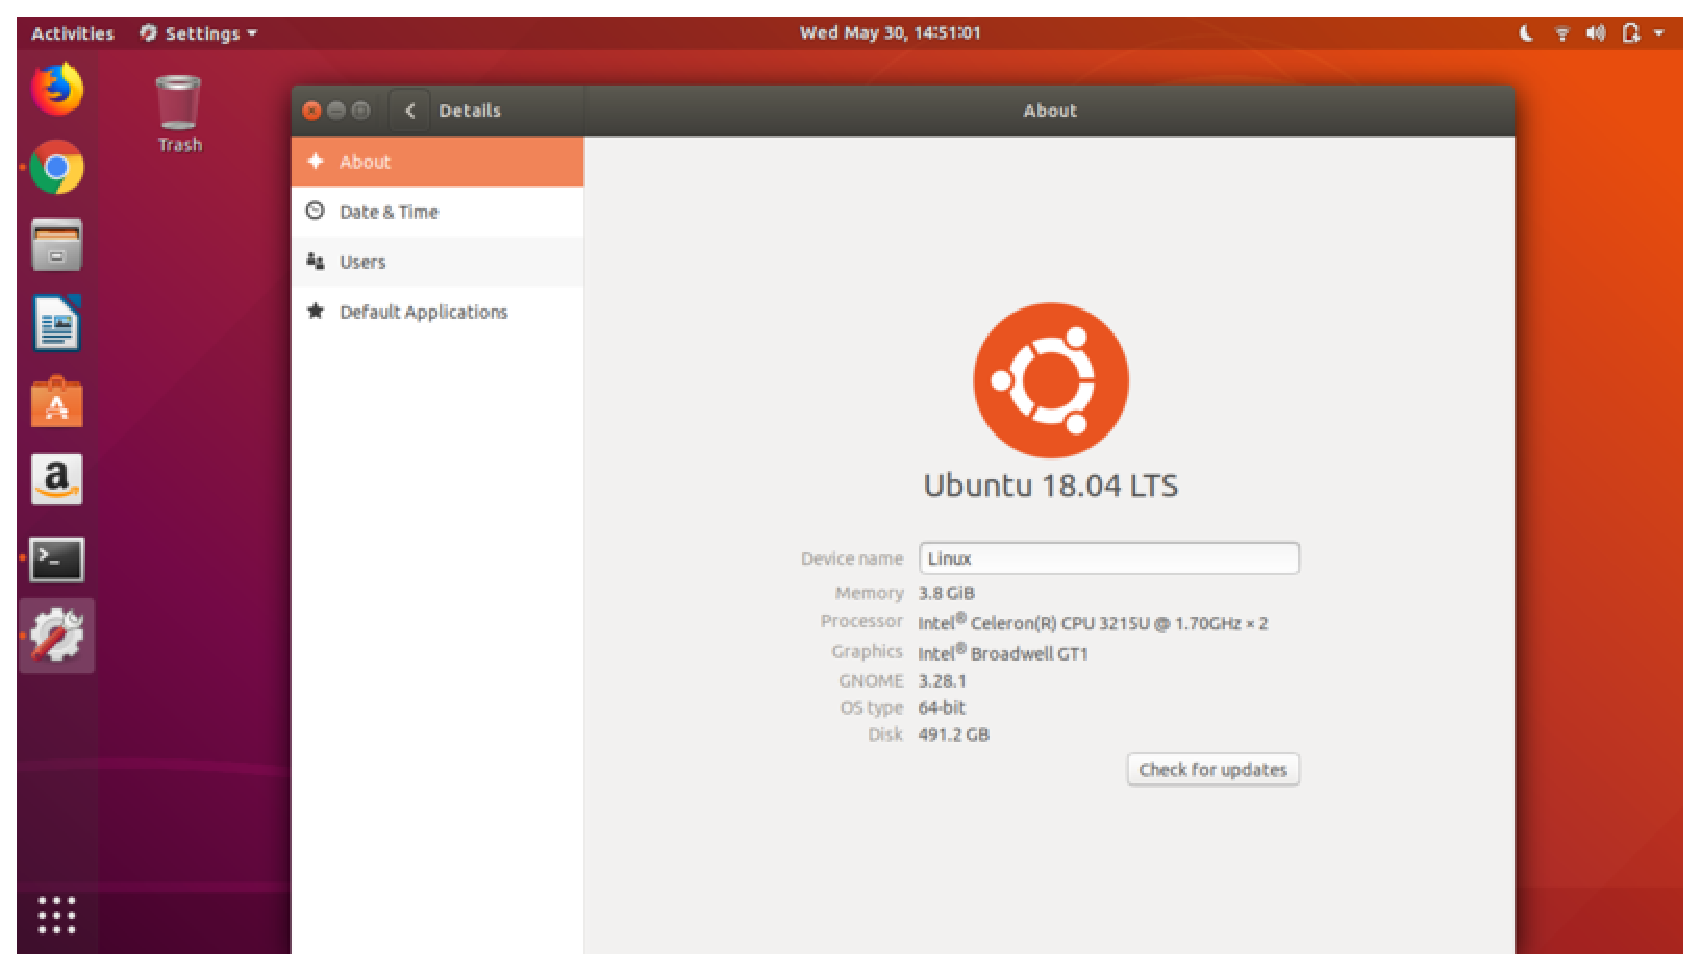
\includegraphics[scale=.5]{Ubuntu-18.04.eps}
%		\caption{Linux Ubuntu version 18.04 desktop.}
%		\label{fig:ubuntu}
%	\end{figure}
%\end{center}

\paragraph{Kali Linux}is a Linux distribution for penetration
testers. It consists of many widely used tools for pentest. This
distribution make it easy to use common tools in a pentest. There are
about 200+ tools in Kali Linux for various stages of a
pentest. Figure~\ref{fig:kali} show a Kali Linux distributions with
tools for penetration testing.

%\begin{center}
%	\begin{figure}[]
%		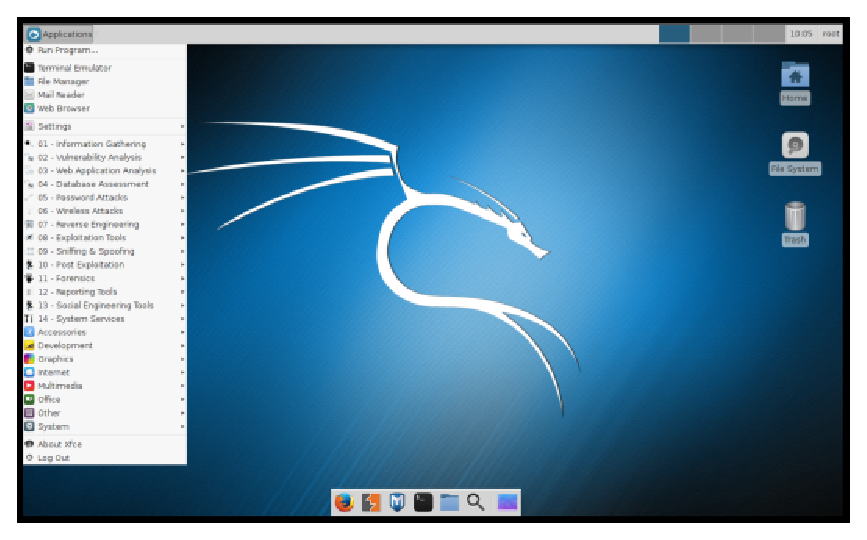
\includegraphics[scale=.5]{kali-linux.eps}
%		\caption{Kali Linux. A Linux distribution for pen testers.}
%		\label{fig:kali}
%	\end{figure}
%\end{center}

\begin{figure*}[!t]
\centering
\subfloat[Kali Linux]{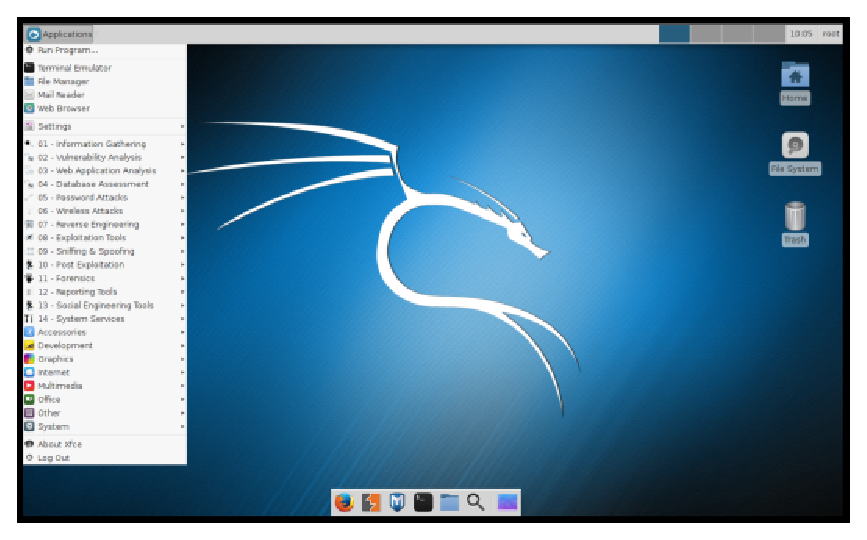
\includegraphics[width=.45\textwidth]{kali-linux.eps}%
\label{fig:kali}}
\hfil
\subfloat[Ubuntu Linux]{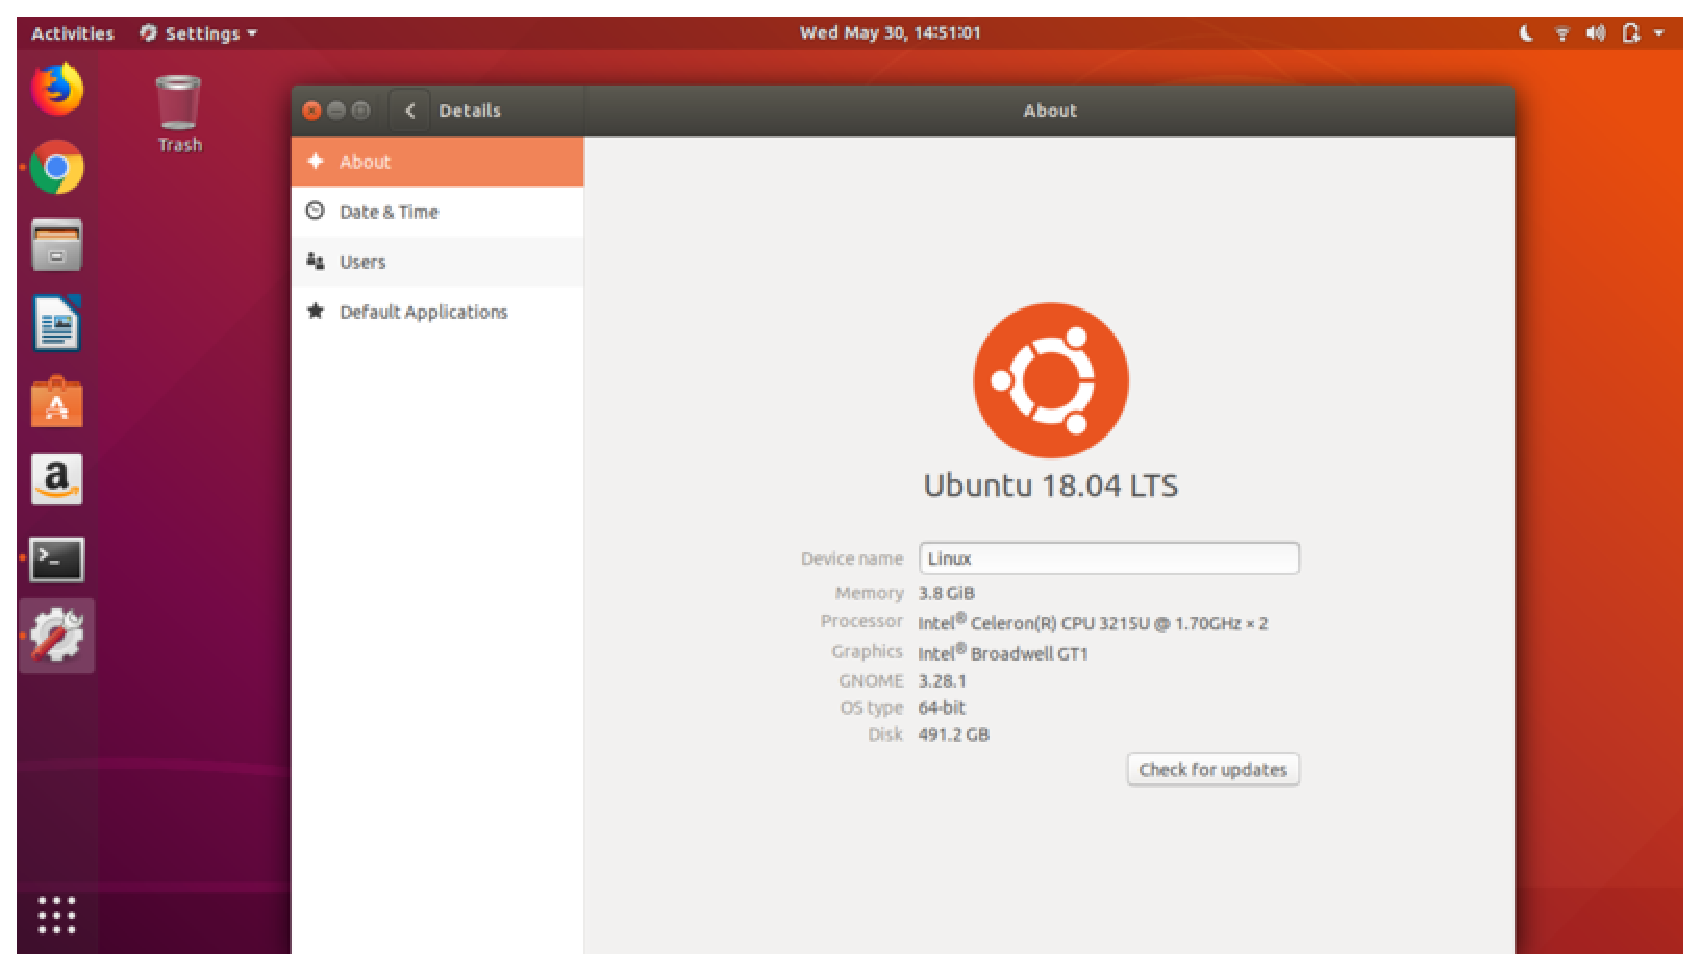
\includegraphics[width=.45\textwidth]{Ubuntu-18.04.eps}%
\label{fig:ubuntu}}
\caption{Example of Linux distributions.}
\label{fig:linux}
\end{figure*}

There exist various approach in installing and using Linux. One of the easiest is to install
Kali Linux on a standalone machine. Another is to install Kali Linux as a dual boot system 
together with Window 10/7. Another approach is to install Kali Linux on a virtual machine such
as VirtualBox or VMware. Another is using docker. And, for more advance user, you can run Kali 
Linux on the cloud, without installing anything on your computer. Please google for more information
if you are interested in installing Kali Linux as your pen test platform.

\index{topics}{docker}


One widely used Linux derivative is Android, an operating system used in 
mobile phone. It is estimated that Android has a market share of about 70\% 
for mobile phone and 30\% for iOS.



\section{git}

\paragraph{git}\cite{loeliger2012} is a source code
management tool. \url{github.com} is a git repository, where
software developers share their software source codes in the
Internet. \url{Github.com} host many open source pen test
tools projects such as \url{metasploit} and \url{nmap}. A
pen tester can clone the repository and install the software
on his machine. With this approach, the pen tester can
always use the latest version of the software.

A pen tester need to clone the repository from \url{github.com}. An
example for such action is given below for cloning \url{nmap}
repository. Figure~\ref{fig:github} show a sample repository at
\url{github.com}.


\verb|git clone https://github.com/nmap/nmap.git|

% https://www.online-convert.com/
% take screen shot in png, convert to eps

%\begin{center}
%	\begin{figure}[ht]
%		\includegraphics[width=.50\textwidth]{github.eps}
%		\caption{github.com}
%	\end{figure}
%\end{center}

\begin{figure}
\centering
\includegraphics[width=.75\textwidth]{github-ui.eps}
\caption{Source code repository at github.com}
\label{fig:github}
\end{figure}

\index{topics}{git}
\index{authors}{Loeliger, Jon}

\section{Python}

\paragraph{Python}\cite{van2007python,lutz2013learning,lutz2010programming}
is a general-purpose, high-level programming language whose design
philosophy emphasizes code readability. Currently, it is widely used
in data science, deep learning and web development and software
development. It has been used to develop tools for pen tests.  There
are many pen test tools written in Python, hosted at
\url{github.com}. An example is \url{Sublist3r}, a tool for network
scanning and reconnaissance \index{topics}{Sublist3r}

\index{topics}{Python}
\index{authors}{Lutz, Mark}

Many processes in a pen test can be automated using Python. We could develop 
new tools for pen tests, automated the
process and discovered new vulnerabilities.


%\section{Raspberry Pi}
%
%\paragraph{Raspberry Pi} is a small single-board computer. It can be used 

\section{Cybersecurity News}

\section{Definitions}

\section{Web resources}

There exist tons of materials related to pen-test online. It is best to adopt
a life long attitude toward pen test where one try to always update oneself
with the latest info about pen test. These are some of useful websites;
\begin{enumerate}
\item \url{https://github.com/enaqx/awesome-pentest}
\item \url{https://github.com/paralax/Awesome-Pentest-1}
\item \url{https://github.com/coreb1t/awesome-pentest-cheat-sheets}
\item \url{https://pen-testing.sans.org/}
\end{enumerate}





\section{Cybersecurity Accreditation}

There are many industry-based certificates that a pen tester
could pursue to enhance marketability and to increase knowledge. One of the 
certification is GPEN (GIAC Penetration Tester) at 
\url{https://pen-testing.sans.org/certification/gpen}, offered by SANS  
Institute. Another is OSCP (Offensive
Security Certified Pen Tester) at \url{https://www.offensive-security.com/}.
Another widely accepted certification is CEH(Certified Ethical Hacking) by 
EC-Council\url{https://www.eccouncil.org/}.

 
\section{Summary}

For a basic skill, a pen tester need to be familiar with Linux, especially Kali
Linux. He also need to know \url{git} and \url{github.com} for pen test tools
repository. For advance pen test, he could learn Python for automation and 
advance exploit.

In summary, pen test is a wide field and there are almost unlimited information
in the Internet. 
\begin{center}
	\begin{figure}[ht]
		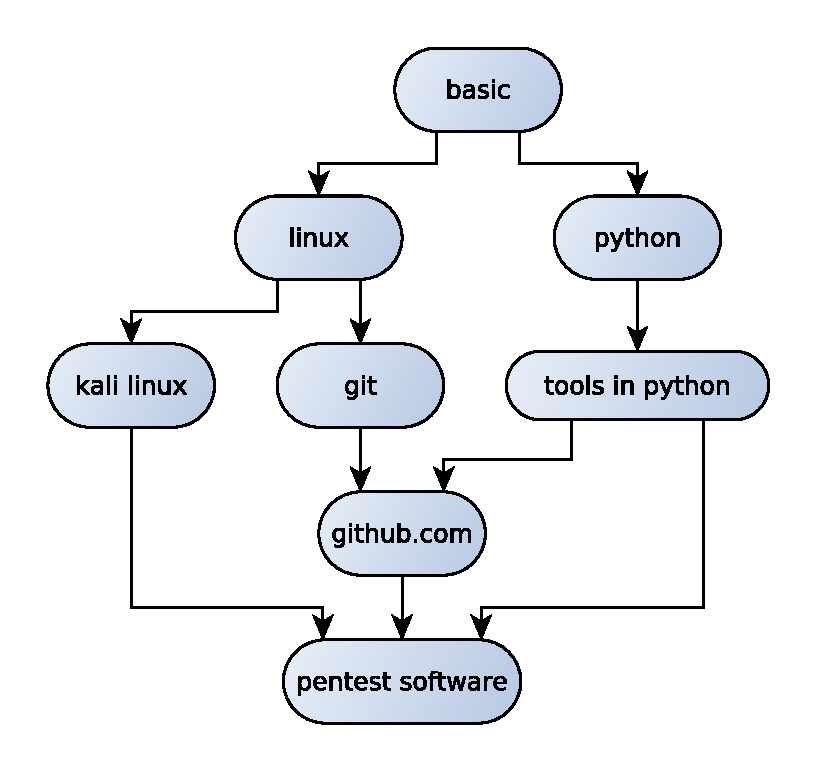
\includegraphics[scale=.75]{tools.eps}
		\caption{Basic tools for pen testers.}
	\end{figure}
\end{center}

\begin{table}[]
    \begin{tabular}{|c|l|c|}
        \hline 
        Tool & Use &  \\ 
        \hline 
        Linux & operating system &  \\ 
        \hline 
        git & software repository &  \\ 
        \hline 
        Python & Programming language. advance pen test &  \\ 
        \hline 
    \end{tabular}
    \caption{Summary of common tools}
    \label{tab:tools}
\end{table}



\chapternotes
 

\chapter{Network Basic}

% based on SANS540

\section{Network}
\section{How Internet works}
\section{IP, DNS}
\section{Web servers}


\chapter{Network}

\section{Reconnaissance}
\section{Scanning}
\section{Enumeration}
\section{Vulnerability Assessment}



\chapter{Web Apps}
\section{Web Apps}
\section{Reconnaissance}
\section{Scanning}
\section{Enumeration}
\section{Vulnerability Assessment}

\chapter{Wireless}



\chapter{Mobile}

\chapter{Server and Desktop}

%\nocite{*}
%\bibliographystyle{mit-chicago}
\bibliographystyle{unsrt}
\bibliography{buku}


\printindex{authors}{Author Index}
\printindex{topics}{Topic Index}

\end{document}


% GPEN 
Exam Certification Objectives

Objectives	Objective Outcome Statement

Advanced Password Attacks
The candidate will be able to use additional 
methods to attack password hashes and authenticate.

Attacking Password Hashes
The candidate will be able to obtain and attack 
password hashes and other password representations.

Escalation and Exploitation
The candidate will be able to demonstrate the 
fundamental concepts of exploitation, data exfiltration from compromised hosts 
and pivoting to exploit other hosts within a target network.

Exploitation Fundamentals
The candidate will be able to demonstrate the 
fundamental concepts associated with the exploitation phase of a pentest.

Metasploit
The candidate will be able to use and configure the Metasploit 
Framework at an intermediate level.

Moving Files with Exploits
The candidate will be able to use exploits to move 
files between remote systems.

Password Attacks
The candidate will understand types of password attacks, 
formats, defenses, and the circumstances under which to use each password 
attack variation. The candidate will be able to conduct password guessing 
attacks.

Password Formats and Hashes
The candidate will demonstrate an understanding of 
common password hashes and formats for storing password data.

Penetration Test Planning
The candidate will be able to demonstrate the 
fundamental concepts associated with pen-testing, and utilize a 
process-oriented approach to penetration testing and reporting.

Penetration Testing with PowerShell and the Windows Command Line
The candidate will demonstrate an understanding of the use of advanced Windows 
command line skills during a penetration test, and demonstrate an understanding 
of the use of advanced Windows Power Shell skills during a penetration test.

Reconnaissance
The candidate will understand the fundamental concepts of 
reconnaissance and will understand how to obtain basic, high level information 
about the target organization and network, often considered information 
leakage, including but not limited to technical and non technical public 
contacts, IP address ranges, document formats, and supported systems.

Scanning and Host Discovery
The candidate will be able to use the appropriate 
technique to scan a network for potential targets, and to conduct port, 
operating system and service version scans and analyze the results.
Vulnerability Scanning	The candidate will be able to conduct vulnerability 
scans and analyze the results.

Web Application Injection Attacks
The candidate will demonstrate an understanding of how injection attacks work 
against web applications and how to 
conduct them.

Web Application Reconnaisance
The candidate will demonstrate an understanding 
of the use of tools and proxies to discover web application vulnerabilities.

XSS and CSRF Attacks
The candidate will demonstrate an understanding of how 
XSS and CSRF attacks work and how to conduct them.

%